\chapter{Modèle conceptuel et logique du schéma décisionnel}\label{chap:modele}

\section{Grains et matrice en bus}
Le modèle suit l'approche Kimball : quatre processus métiers (consultation, hospitalisation, décès, satisfaction), chacun modélisé par une table de faits entourée de dimensions. Le grain retenu est le plus fin disponible dans les sources.

\begin{table}[!htbp]\small
\caption{Processus, grain et type de fait}\label{tab:grains}
\begin{tabularx}{\linewidth}{@{}L{2.5cm}L{4.2cm}L{2.5cm}Y@{}}
\toprule\entete\textbf{Processus} & \textbf{Grain} & \textbf{Type} & \textbf{Besoins couverts}\\\midrule
Consultation & Une consultation (\code{Num\_consultation}) & Transactionnel & Taux de consultation par établissement, par diagnostic, par professionnel \\
Hospitalisation & Un séjour (entrée et durée) & Transactionnel & Taux d'hospitalisation global, par diagnostic, par sexe et âge \\
Décès & Un acte de décès dédoublonné & Transactionnel & Nombre de décès par région \\
Satisfaction & Un résultat d'indicateur par établissement et campagne & Instantané annuel & Taux de satisfaction par région \\
\bottomrule
\end{tabularx}
\end{table}

Quatre faits distincts sont nécessaires car les grains sont incompatibles : le décès n'a pas de patient (open data sans appariement), le résultat HAS est un agrégat publié. Les dimensions conformes (tableau~\ref{tab:bus}) relient les quatre faits pour les analyses croisées.

\begin{table}[!htbp]\small\centering
\caption{Matrice en bus (processus $\times$ dimensions)}\label{tab:bus}
\setlength{\tabcolsep}{3.5pt}
\begin{tabular}{@{}lcccccccccccc@{}}
\toprule\entete
\textbf{Processus} & \rotatebox{70}{\textbf{Date}} & \rotatebox{70}{\textbf{Patient}} & \rotatebox{70}{\textbf{Sexe}} & \rotatebox{70}{\textbf{Tranche d'âge}} & \rotatebox{70}{\textbf{Établissement}} & \rotatebox{70}{\textbf{Géographie}} & \rotatebox{70}{\textbf{Diagnostic}} & \rotatebox{70}{\textbf{Professionnel}} & \rotatebox{70}{\textbf{Mutuelle}} & \rotatebox{70}{\textbf{Acte}} & \rotatebox{70}{\textbf{Campagne}} & \rotatebox{70}{\textbf{Indicateur}}\\\midrule
Consultation & \checkmark & \checkmark & \checkmark & \checkmark & \checkmark & \checkmark\textsuperscript{E} & \checkmark & \checkmark & \checkmark & \checkmark & & \\
Hospitalisation & \checkmark{}\,$\times$2 & \checkmark & \checkmark & \checkmark & \checkmark & \checkmark\textsuperscript{E} & \checkmark & & & & & \\
Décès & \checkmark & & \checkmark & \checkmark & & \checkmark\textsuperscript{D} & & & & & & \\
Satisfaction / qualité & \checkmark\textsuperscript{R} & & & & \checkmark & \checkmark\textsuperscript{E} & & & & & \checkmark & \checkmark \\\midrule
\textit{Conforme ?} & oui & oui & oui & oui & oui & oui$^{\ast}$ & oui & non & non & non & non & non \\
\bottomrule
\end{tabular}
\par\smallskip\raggedright\small $\times$2 : double rôle (entrée, sortie). \textsuperscript{R} : \code{date\_reference\_sk}, 1\textsuperscript{er} janvier de l'année des données. Rôles de \code{dim\_geographie} : \textsuperscript{E} lieu de l'établissement, \textsuperscript{D} lieu du décès. $^{\ast}$ Résidence du patient et géographie de l'établissement reprennent ses codes.
\end{table}

\section{Modèle conceptuel de données (MCD)}
Le MCD Merise est présenté en deux vues reliées par l'entité ÉTABLISSEMENT (figures~\ref{fig:mcd-a} et \ref{fig:mcd-b}). Règles : RG-M01, une consultation a un seul patient, professionnel, diagnostic et mutuelle ; RG-M02, un séjour a un seul patient, établissement et diagnostic ; RG-M03, un professionnel exerce dans 0 à n établissements ; RG-M04, un établissement est dans 0 ou 1 commune ; RG-M05, un décès survient dans une commune ou à l'étranger ; RG-M06, l'association ternaire MESURER devient \code{fait\_indicateur\_qualite}.

\begin{figure}[!htbp]\centering
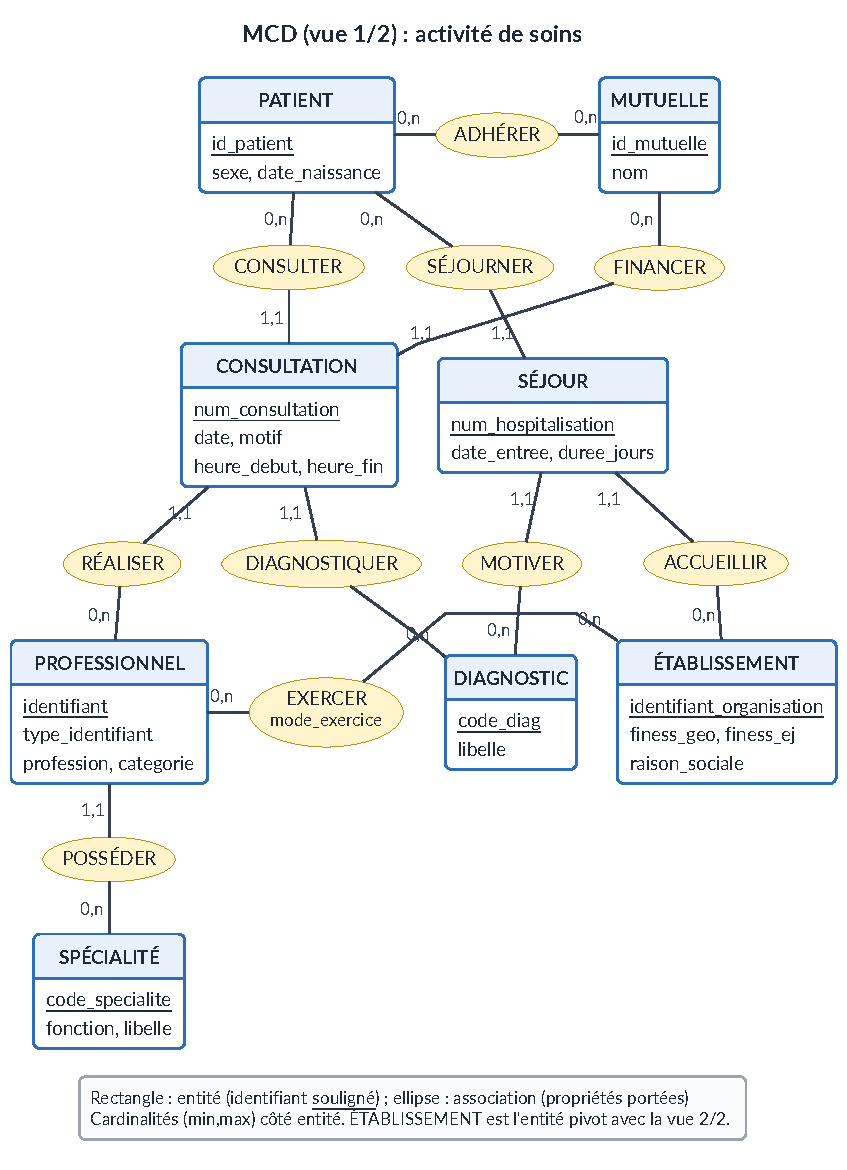
\includegraphics[width=0.78\linewidth]{figures/10a_mcd_activite.pdf}
\caption{MCD (vue 1/2), activité de soins}\label{fig:mcd-a}
\end{figure}

\begin{figure}[!htbp]\centering
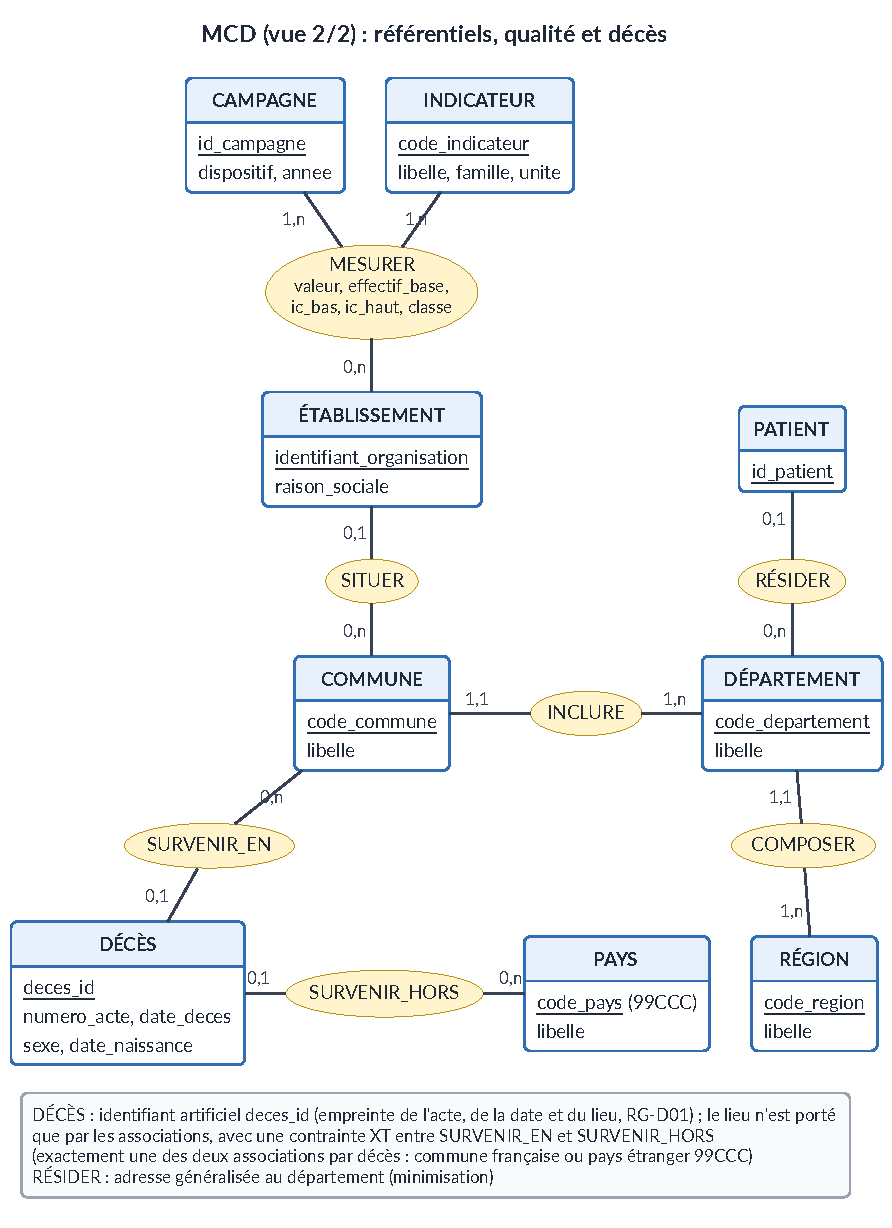
\includegraphics[width=0.78\linewidth]{figures/10b_mcd_referentiels.pdf}
\caption{MCD (vue 2/2), référentiels, qualité et décès}\label{fig:mcd-b}
\end{figure}

\section{Modèle logique : schémas en étoile}\label{sec:logique}
La constellation (figure~\ref{fig:constellation}) montre les quatre faits et les dimensions partagées. Le dictionnaire complet (\nbTables{} tables, \nbColonnes{} attributs, \nbFK{} clés étrangères) est en annexe~\ref{sec:dictionnaire}.

\begin{figure}[!htbp]\centering
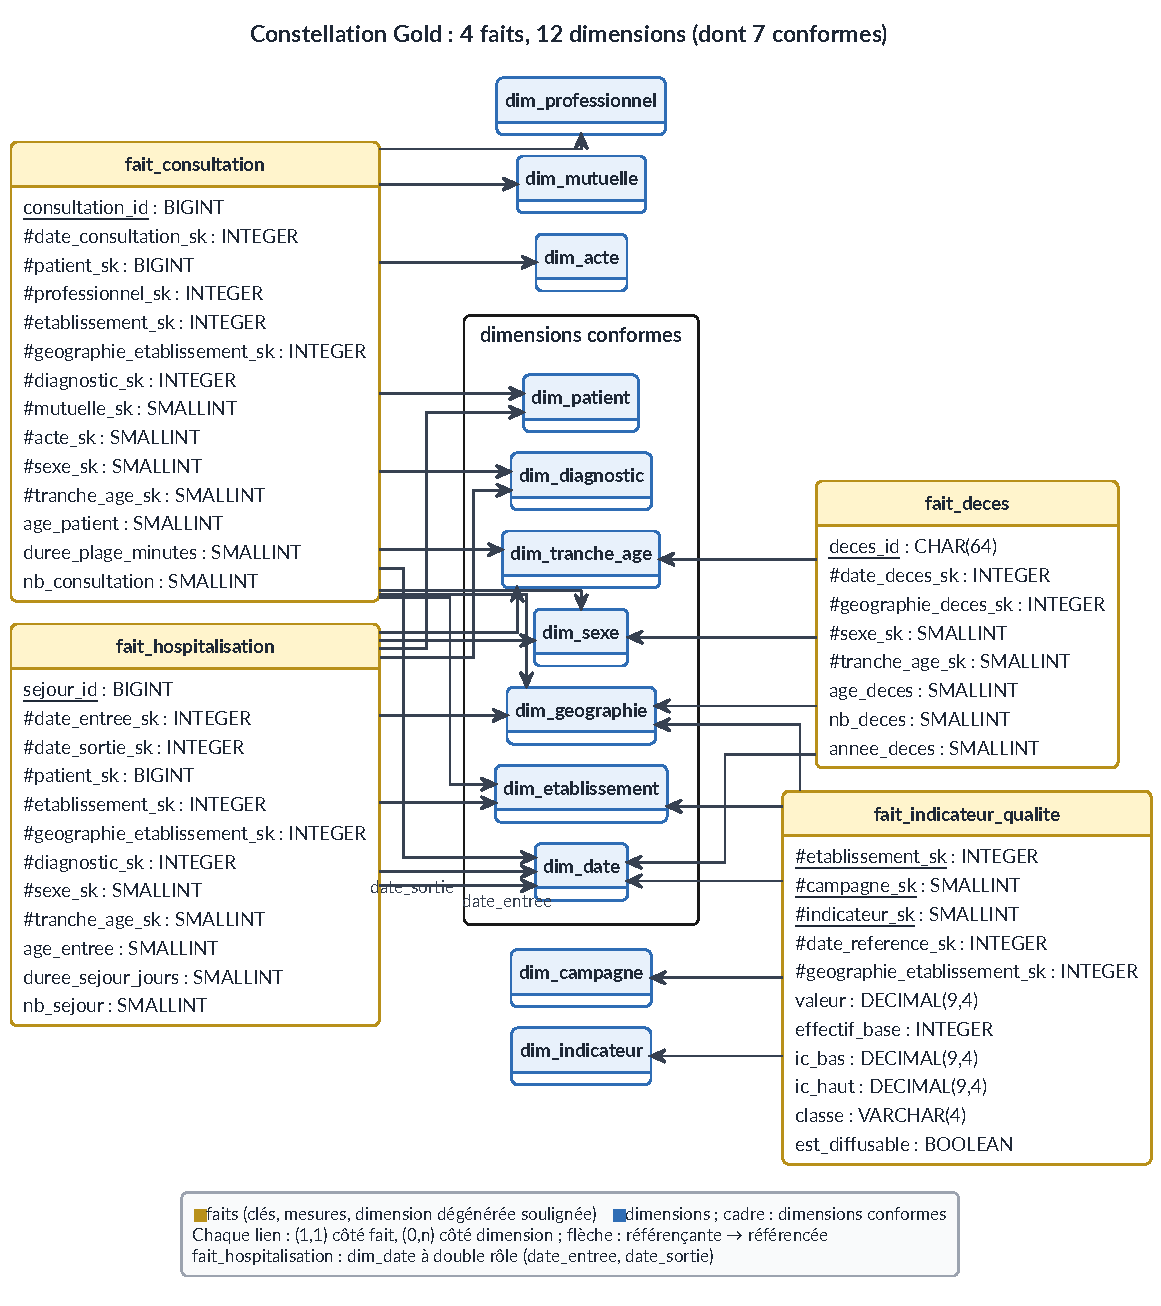
\includegraphics[width=\linewidth,height=0.62\textheight,keepaspectratio]{figures/05_constellation.pdf}
\caption{Constellation de faits de la couche Gold}\label{fig:constellation}
\end{figure}

\begin{figure}[!htbp]\centering
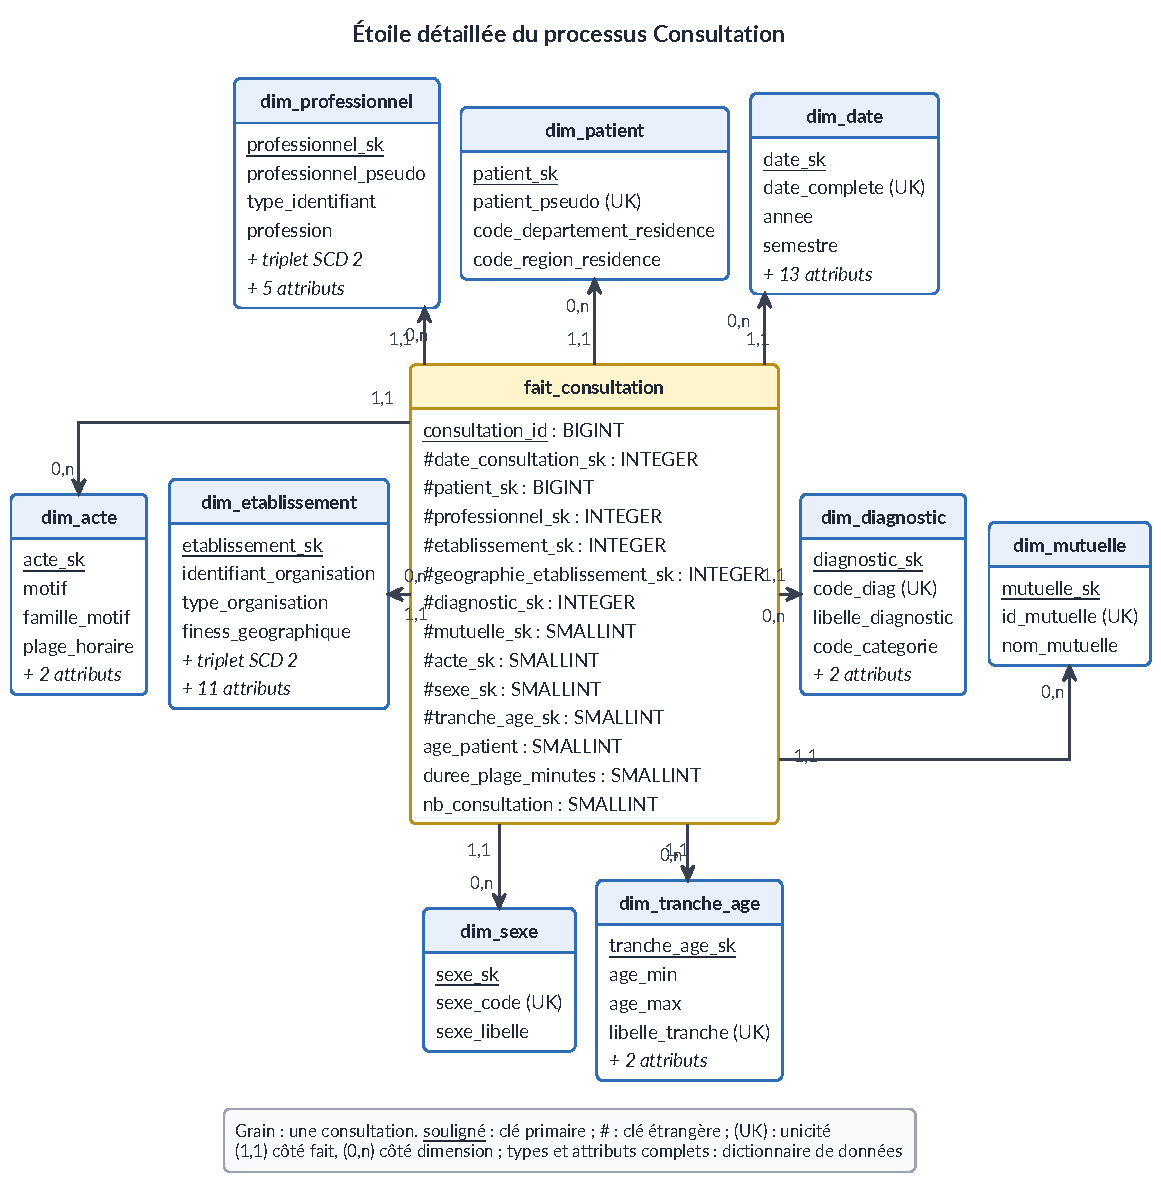
\includegraphics[width=0.92\linewidth]{figures/06_etoile_consultation.pdf}
\caption{MLD du processus Consultation (schéma en étoile)}\label{fig:etoile-cons}
\end{figure}

\textbf{Cardinalités.} Toute clé étrangère d'un fait est non nulle (membres spéciaux) et référence une seule ligne de dimension : cardinalité (1,1) côté fait, (0,n) côté dimension, soit une relation N:1 (tableau~\ref{tab:cardinalites}). Pour les dimensions SCD~2, la clé durable porte 1 à $n$ versions ; le fait pointe la version en vigueur à la date de l'événement.

\begin{table}[!htbp]
\caption{Cardinalités des clés étrangères par étoile, (1,1) côté fait et (0,n) côté dimension}\label{tab:cardinalites}
{\small\begin{tabularx}{\linewidth}{@{}L{4.6cm}Y@{}}
\toprule\entete\textbf{Fait (étoile)} & \textbf{Dimensions référencées (préfixe \code{dim\_}), chacune en N:1}\\\midrule
\code{fait\_consultation} (10 FK) & \code{date}, \code{patient}, \code{professionnel}, \code{etablissement}, \code{geographie}, \code{diagnostic}, \code{mutuelle}, \code{acte}, \code{sexe}, \code{tranche\_age} \\
\code{fait\_hospitalisation} (8 FK) & \code{date} $\times$2, \code{patient}, \code{etablissement}, \code{geographie}, \code{diagnostic}, \code{sexe}, \code{tranche\_age} \\
\code{fait\_deces} (4 FK) & \code{date}, \code{geographie}, \code{sexe}, \code{tranche\_age} \\
\code{fait\_indicateur\_qualite} (5 FK) & \code{etablissement}, \code{campagne}, \code{indicateur}, \code{date}, \code{geographie} \\
\bottomrule\end{tabularx}}
\end{table}

\section{Clés de substitution et membres spéciaux}
Chaque dimension possède une clé entière automatique (suffixe \code{\_sk}), distincte de la clé source, stable d'un chargement à l'autre. \code{dim\_date} utilise la clé \code{AAAAMMJJ}. Une clé étrangère de fait n'est jamais \code{NULL} : elle pointe vers un membre spécial.

\begin{table}[!htbp]\small
\caption{Membres spéciaux}\label{tab:membres}
\begin{tabularx}{\linewidth}{@{}L{0.9cm}L{3.2cm}L{4.3cm}Y@{}}
\toprule\entete\textbf{Clé} & \textbf{Libellé} & \textbf{Dimensions} & \textbf{Usage}\\\midrule
$-1$ & Inconnu & Toutes & Valeur absente dans la source. \\
$-2$ & Non applicable & \code{dim\_date} & Attribut sans objet. \\
$-3$ & Hors référentiel & \code{dim\_diagnostic}, \code{dim\_geographie}, \code{dim\_etablissement} & Code présent mais absent du référentiel ; valeur brute gardée en Silver. \\
$-4$ & Non déterminable & \code{dim\_etablissement} & La règle de dérivation ne conclut pas (consultation sans activité rattachée). \\
\bottomrule
\end{tabularx}
\end{table}

\begin{table}[!htbp]\small
\caption{Historisation des dimensions (SCD)}\label{tab:scd}
\begin{tabularx}{\linewidth}{@{}L{3.0cm}L{3.2cm}Y@{}}
\toprule\entete\textbf{Dimension} & \textbf{Type} & \textbf{Justification}\\\midrule
\code{dim\_etablissement} & 2 (raison sociale, commune, entité juridique, catégorie) & Un acte reste attribué à l'établissement tel qu'il était ; clé durable \code{identifiant\_organisation}. \\
\code{dim\_professionnel} & 2 (profession, spécialité, mode d'exercice) & Version en vigueur à la date de l'acte ; clé durable \code{professionnel\_pseudo}. \\
\code{dim\_patient}, référentiels & 1 & Valeur actuelle. \\
Date, sexe, tranche, acte, campagne & Statique & Générées ou observées. \\
\bottomrule
\end{tabularx}
\end{table}

\textbf{Additivité} : les comptes (\code{nb\_*}) et durées sont additifs ; âges et scores ne le sont pas (moyenne pondérée par \code{effectif\_base}) ; les patients distincts se recomptent, jamais ne se somment.
